% Needed packages
\documentclass[a4paper, 10pt, english, onecolumn]{article}
\usepackage[english]{babel}
\usepackage[cm]{fullpage}
\usepackage{cite}
\usepackage{anysize}
%\usepackage[compact]{titlesec}
\usepackage{graphicx}
\usepackage{stfloats}
\usepackage{listings}
\usepackage{hyperref}

\usepackage{amssymb,amsmath}
\usepackage{algorithmicx}
%\usepackage{algorithmic}
\usepackage{algorithm}
\usepackage[noend]{algpseudocode}

% for coloring individual cells in a table
\usepackage[table]{xcolor}
%\usepackage{pgfgantt}

%\newcommand{\keywords}[1]{\par\noindent 
%{\bf Keywords\/}. #1}

% Margins & Headers
\marginsize{2.5cm}{2.5cm}{3.0cm}{2.0cm}
\columnsep 0.4in
\footskip 0.4in 
\usepackage{changepage}

% E-mail formatting
\usepackage{color,hyperref}
    \catcode`\_=11\relax
    \newcommand\email[1]{\_email #1\q_nil}
    \def\_email#1@#2\q_nil{
      \href{mailto:#1@#2}{{\emailfont #1\emailampersat #2}}
    }
    \newcommand\emailfont{\sffamily}
    \newcommand\emailampersat{{\color{red}\small@}}
    \catcode`\_=8\relax 
	
% List modifications
\newenvironment{packed_item}{
\begin{itemize}
  \setlength{\itemsep}{1pt}
  \setlength{\parskip}{0pt}
  \setlength{\parsep}{0pt}
}{\end{itemize}}

\newenvironment{packed_enum}{
\begin{enumerate}
  \setlength{\itemsep}{1pt}
  \setlength{\parskip}{0pt}
  \setlength{\parsep}{0pt}
}{\end{enumerate}}

% ### Mathematics ###
\newcommand{\bpm}{\begin{pmatrix}}
\newcommand{\epm}{\end{pmatrix}}

\newcommand{\bbm}{\begin{bmatrix}}
\newcommand{\ebm}{\end{bmatrix}}

\newcommand{\bsm}{\bigl( \begin{smallmatrix}}
\newcommand{\esm}{ \end{smallmatrix} \bigl)} 

\newcommand{\mbf}{\mathbf}

% ### Matrices and Vectors ###
\newcommand{\mtx}[1]{\ensuremath{\boldsymbol{#1}}}
\newcommand*\Let[2]{\State #1 $\gets$ #2}

% ### Sets ###
\newcommand{\set}[1]{\ensuremath{\mathcal{#1}}}

% ### Other ###

\newcommand{\transpose}{^{T}}
\newcommand{\inv}{^{-1}}
\newcommand{\pseudoinv}{^{+}}

% ### Hyphenation ###
\hyphenation{a-na-ly-sis}

% ### dots at the end of arrows and lines ###

\def \orightarrow {\circ\hspace{-0.42em}\rightarrow}
\def \oleftarrow {\leftarrow\hspace{-0.42em}\circ}
\def \orightline {\circ\hspace{-0.16em}-}
\def \oleftline {-\hspace{-0.16em}\circ}
\def \oline {\circ\hspace{-0.38em}-\hspace{-0.4em}\circ}
\def \srightarrow {\text{\textasteriskcentered}\hspace{-0.62em}\rightarrow}
\def \sleftarrow {\leftarrow\hspace{-0.62em}\text{\textasteriskcentered}}
\def \srightline {\text{\textasteriskcentered}\hspace{-0.16em}-}
\def \sleftline {-\hspace{-0.40em}\text{\textasteriskcentered}}
\def \sline {\text{\textasteriskcentered}\hspace{-0.38em}-\hspace{-0.4em}\text{\textasteriskcentered}}
\def \soline {\text{\textasteriskcentered}\hspace{-0.16em}-\hspace{-0.4em}\circ}
\def \osline {\circ\hspace{-0.38em}-\hspace{-0.16em}\text{\textasteriskcentered}}

% ############## End Macros ##############


% Title
\title{\fontfamily{phv}\selectfont{Causal Discovery methods for Effective Connectivity}}
\author{
  \textbf{R. Janssen} - \href{mailto:ramon.janssen@student.ru.nl}{ramon.janssen@student.ru.nl} \\
  \textbf{T. de Ruijter} - \href{mailto:t.deruijter@student.ru.nl}{t.deruijter@student.ru.nl}\\
%  \textbf{T. Claassen} - \href{mailto:tomc@cs.ru.nl}{tomc@cs.ru.nl}\\
%  \textbf{M. Hinne} - \href{mailto:mhinne@cs.ru.nl}{mhinne@cs.ru.nl}
}

\date{\fontfamily{ptm}\selectfont{\small{\bfseries{\today - Radboud
Universiteit Nijmegen}}}\\[0.5cm]\rule{\linewidth}{0.3mm}}

\begin{document}

\maketitle

\setlength{\parindent}{0.0cm}
\setlength{\parskip}{0.25cm}

\begin{abstract}
% TODO: Add abstract. Look at slides Peter to see what is asked.
\end{abstract}


\section{Introduction}

\paragraph{Motivation}
The brain and particularly the human brain have been studied for hundreds of years.
Today, the secrets of our brains still are one of the most sought-after.
The techniques however have changed.
We have come a long way since the time of Phrenology, the pseudoscience based attempting to derive cognitive ability and personality from measurements of the skull or, post-mortem, the brain.
Advanced measurement methods exist that allow scientists to peek inside brains that give a coarse but broad overview without opening a single skull.

Of particular interest are causal relations between brain regions and cognitive and bodily functions.
The question if brain region X is functionally or structurally connected to brain region Y and whether these are causally related is still highly relevant; it is the main question of the present-day scientific field of brain connectivity.
Understanding brain structure implies understanding more about the brain as a whole.

Not surprisingly, brain connectivity also finds applications in medicine.
Neuro-degenerative diseases such as Alzheimer's disease, Parkinson's disease, dementia, Amyotrophic lateral sclerosis (ALS) have all been shown to severely alter brain connectivity. %TODO: Citation needed.
Better methods for analysing connectivity could lead to more insight in these diseases.

The field of brain connectivity finds its roots in the early 1990s \cite{friston1993functional, friston1994}, though because of more recent developments in the field of Artificial Intelligence and Machine Learning it is possible to do more thorough analysis \cite{vandenheuvel2010}.
One type of connectivity analysis involves finding how brain region X causes what region Y does. This is called \emph{effective connectivity}.
More concretely: how does the measured fMRI signal, representing an underlying neuronal process, determine what other neuronal processes are activated.
Research regarding effective is relatively new and its application still faces many challenges that require further research \cite{ramsey2010}.
The directed character in effective connectivity seems similar to traditional causal relations.
In what follows, we suggest to use causal discovery methods for deriving effective connectivity.

\paragraph{Problem statement}
This project seeks to utilise the strengths of current state-of-the-art causal discovery methods by applying them to resting state brain fMRI data in order to find new applicable methods for determining causal patterns in the human brain.

The work by \cite{ramsey2010} addresses several problems causal analysis in fMRI analysis suffers from.
Methods in causal discovery have high computational costs, making it nearly impossible to calculate networks with more than hundreds of nodes.
Another important fact is that fMRI Analysis indirectly measures brain activity.
Brain models that do not account for possible latent - indirect - sources within the brain or the shortcomings of fMRI may suffer from noise, fail to capture underlying patterns or draw erroneous conclusions.
Solutions to this particular problem have been proposed that do account for latent sources \cite{ramsey2010, waldorp2011}.
Another problem is the strong diversity between subjects.
Every brain is inherently different, making it non-trivial to combine subject data or even draw conclusions across subjects.
Even within a single brain it changes how different areas react over time.

Several methods for finding effective connectivity already exist \cite{mclntosh1994, harrison2003, friston2003, roebroeck2005}.
However, using more generally applicable causal discovery methods has not been elaborated on much.
Also, none of these provide a measure of uncertainty.
It is a fact that there are errors in any graph produced.
This is inherent to the methods and the coarseness of the measurements.
As there is no standard baseline to compare results with, a measure of uncertainty would be highly preferable.
A framework for such a probabilistic approach is introduced in \cite{claassen2012}.

We would like to know whether applying such methods, such as the approach introduced in \cite{claassen2012}, or a standard approach such as the PC-algorithm \cite{spirtes2000}, named after its authors \textbf{P}eter Spirtes and \textbf{C}lark Glymour, can solve some of the difficulties effective connectivity suffers from.

% Structure of the rest of proposal
In the remainder of this proposal we briefly discuss some necessary background knowledge on connectivity and methods, we then discuss our strategy and finally we present a time-plan overview.

\section{Theory}

\subsection{Causal discovery}
An approach for finding effective connectivity may be found in the domain of causal discovery.
A causal discovery method uses data about events to determine which of these events are correlated, and additionally, it attempts to determine which events cause which.
The definition of a causal relation is not trivial \cite[p.20]{spirtes2000} and the relevant principles will be covered in this section.
In our context, the causal discovery methods which have been used aim at inferring a Bayesian network or Directed Acyclic Graph (DAG).
These can be interpreted from a probabilistic and a causal perspective.
In our case, we consider graphs that also include non-directed edges, a so called Partial DAG (PDAG).

Under the causal interpretation, a PDAG $G$ each variable is represented by a node and correlations between variables are represented by edges between those nodes.
If such an edge exists between two variables $X$ and $Y$, this is denoted as $X - Y$.
A causal relation is denoted with directed edges; $X \rightarrow Y$ implies that $X$ is a direct cause of $Y$.
It is also said that $X$ is the parent of $Y$, and $Y$ is the child of $X$. 
When there is a directed path $X \rightarrow Z_1 \rightarrow Z_2 \dots \rightarrow Y$, $X$ is said to be an ancestor of $Y$ and $Y$ is a descendant of $X$.
An ancestor is an (possibly indirect) cause of its descendant.

% TODO: Add example of a Bayesian network.
%Image {plaatje!} shows an example of a Bayesian network.

A causal discovery method attempts at finding a real-world Bayesian network.
The human brain is immensely complex and contains a computationally intractable amount of neurons to model.
As such, we represent our real-world, underlying Bayesian network with a much simpler model.
Such a model contains a reduced number of variables in order to remain tractable and to visually interpret model results.

An important principle for our approach is that of conditional dependence.
The dependency of two variables might depend on the value of a third variable (or possibly even more variables).
This principle is best demonstrated with an example.
When two variables, such as two switches being turned off or on, both cause a light bulb to glow, the two switches might not be dependent.
Whether one switch is turned on or off does not cause the other to switch on or off.
However, when the light bulb is glowing, the switches do become dependent.
If one switch is off, the other one is probably on.
Or in other words, one switch being turned on decreases the chance of the other switch being turned on.
In this case, we conclude that the switches are conditionally dependent given that the light bulb is turned on.
More generally, two variables $X$ and $Y$ can be conditionally dependent on a set of other variables $S$. % het juiste latex-symbooltje vinden :(

A similar principle is conditional independence.
If two variables are generally dependent, they can still be independent given a third variable.
An example of this is when a variable $X$ has two children $Y$ and $Z$.
$Y$ and $Z$ are generally dependent, as they share a common cause or \emph{confounder} or \emph{confounder} $X$;
When $X$ does not vary, $Y$ and $Z$ lose their confoundernd they lose their dependency.
As such, $Y$ and $Z$ are independent given \{$X$\}.
In real-world data, independence can be found with methods such as the Fisher-Z-test. 

We define a trail as a set of edges which would make up a path if those edges would be undirected.
We can now define directional separation, or d-separation.
Two nodes $X$ and $Y$ are d-separated given a set of nodes $S$ (with $X, Y \notin S$) if there is a trail from $X$ to $Y$ for which at least one of the following holds:
\begin{itemize}
\item The trail contains a structure $a \rightarrow b \rightarrow c$ such that $b$ is in $S$.
\item The trail contains a structure $a \leftarrow b \rightarrow c$ such that $b$ is in $S$.
\item The trail contains a structure $a \rightarrow b \leftarrow c$ (in which $b$ is called a collider) such that $b$ and its descendants are not in $S$.
\end{itemize}
If $X$ and $Y$ are d-separated given $S$, $S$ is called a separating set of $X$ and $Y$. Every two independent variables have a separating set; if they are unconditionally independent, this is the empty  set.

\subsection{Assumptions about the structure}
In theory, every deterministic real-world situation must be described by some Bayesian model, as all situations conform to causality.
But the underlying real-world data such as the measured brain activity used in this analysis usually does not conform to a simple model.
Assumption can be made about the model to make it easier to infer it, but this increases the risk of drawing false conclusions.

One assumption that can be made about the model is that of causal sufficiency. 
When it is assumed that the model fully describes the real network, so-called V-structures can be concluded. 
When there is a structure $X - Y - Z$, in which $X$ and $Z$ are not connected, the only possible orientation of the connections is $X \rightarrow Y \leftarrow Z$. % TODO: extra uitleg, d-separation?
An approach to finding a model is therefore to find all V-structures and orient them in this way.

However, it is very unlikely that all events which are relevant for the causal graph are measured; 
even with high temporal and spatial resolutions, the entire fysiology of the brain is too complex to capture.
Latent variables are nodes which are present in the underlying Bayesian graph, but which are not measured.
The complex reality might be very similar to a simple model based on the measured data, but it might also be very different.
This correctness of the data is called causal faithfulness.
When there is a structure $X \leftarrow L \rightarrow Y$ in which $L$ is a latent variable, an edge between $X$ and $Y$ might be found while the these two nodes have no direct ancestor/descendant-relation between them;
They might be related through a confounder, which is indicated as $X \leftrightarrow Y$.
As such, for a V-structure for which the underlying Bayesian network has latent variables, a directed edge $X \rightarrow Y$ or $X \leftarrow Y$ would be erroneous. 
As such, the way of describing V-structures might not draw false conclusions, depending on the causal faithfulness. 
A weaker conclusion is that a V-structure should be oriented as $X \orightarrow Y \oleftarrow Z$, in which the circles at the end of an edge mean that the form of this end is not yet know; an arrow $\orightarrow$ might be a simple arrow $\rightarrow$ or a double arrow $\leftrightarrow$.

\subsection{The PC-algorithm}

\subsection{Informal description}
The PC algorithm as used for these experiments is the version which is modified to handle latent variables, as also described by Spirtes, Glymour and Scheines \cite{spirtes2000}, pages 165-167.
For finding directed edges, the PC-algorithm first finds the undirected structure.
For each two nodes $X$ and $Y$ which are not neighbours in this structure, it also finds a minimal separating set, which is the smallest set acting as a separated set.
This is done by first assuming all nodes are connected, and then testing all pairs of nodes for independence.

The independence of $X$ and $Y$ is tested given a subset of neighbours of $X$ or $Y$ (the number of neighbours decreases while edges are removed), using the fisher-Z-test.
If such an independence is found, this subset is a separating set of $X$ and $Y$ and they are not connected.
If no such an independence is found, they are connected.
To find the minimal separating set, all subsets of neighbours are traversed in order of size; the first separating set which is found, is the minimal one.

After the structure and separating sets have been found, the PC-algorithm attempts to orient the edges.
After Spirtes et al, we use a star-symbol at the end of an edge to denote that any mark may be present: an arrowhead, an "o" or an empty mark.
When an edge is oriented as an edge with a star, this denotes that this end is not changed.
A set of rules for finding a causal relation between nodes, using the undirected graph, are used in the PC-algorithm. Multiple variations of this algorithm are described by Spirtes, Glymour and Scheines \ref{?}. For this analysis, we have used the "modified pc algorithm" which does not assume causal sufficiency, and thus is able to handle latent variables.

The first of these rules attempts to find and orient unshielded triples.
A triple $<X, Y, Z>$ is considered unshielded if $X \sline Z$, $Y \sline Z$ and in which $X$ and $Y$ are (possibly conditially) independent.
As $X$ and $Y$ are independent, they have a separating set $S$ (if they are unconditially independent, $S$ is the empty set).
If $Z$ is not in $S$, then the only possible causal relation within this structure can be that of a so-called V-structur; the edges can be oriented as $X \srightarrow Z \sleftarrow Y$.

After this rule which finds V-structures, the other rules are applied in no particular order. These rules are based on arrows that have already been found.
\begin{itemize}
\item If there is an edge $X \sline Y$, and if there is a directed path from $X$ to $Y$, then $X \sline Y$ can be oriented as $X \srightarrow Y$.
\item If there are edges $X \srightarrow Y$ and $Y \sleftline Z$, if the latter is not an edge $Y \sleftarrow Z$, and if $X$ and $Z$ are not connected, orient $Y \sline Z$ as $Y \rightarrow Z$. 
\end{itemize}


\subsection{Brain Connectivity}

%Question: should this be included?
\subsubsection{Functional connectivity}
Functional connectivity describes the statistical dependence of neuronal activity between different brain regions \cite{friston1993functional}.
This gives an insight in the organisation of the brain.
Functional connectivity is strongly time-dependent, as activity changes rapidly providing and fMRI has a low temporal resolution.
This means measured dependencies can be the result of statistical noise.
Functional connectivity can be deduced by fMRI measurement of brains in resting-state \cite{Lowe2000, doria2010, Bullmore2009}.
Resting state indicates that subjects are instructed to relax without thinking of anything in particular to stimulate spontaneous brain activity.

\subsubsection{Structural connectivity}
Structural connectivity is defined as the mapping of anatomical - neural - paths in the brain between different brain regions \cite{friston1994}.
This is strongly related with functional connectivity: regions can only be functionally connected if there is a structural relation between them \cite{cabral2012}.
This intuitive relation can be demonstrated empirically \cite{vandenheuvel2009}.
Structural connectivity is less time dependent as it involves mappings of anatomical connections opposing temporal activity patterns.

Hinne et al. \cite{hinne2013} proposed a Bayesian method for estimating structural networks based on Diffusion Weighted MRI (DWI) and probabilistic Tractography.
The location of white-matter tracts does not become immediately clear from imagery alone.
Other methods rely on thresholds to estimate location of said tracts.
The proposed method results in a measure of uncertainty about where a hypothesised connection will terminate and so provides a clearly interpretable network structure as result.

\subsubsection{Effective connectivity}
In contrast to functional and structural connectivity, effective connectivity takes into account the cause and effect of relations.
It has been described as ``the influence one neural system exerts over another'' \cite{friston1994}.
Effective connectivity indicates which brain regions stimulate other regions.
Time series need to be analysed to infer effective connectivity as cause and effect can be deduced from which event precedes which. 
It is possible to infer effective connectivity from structural and functional connectivity \cite{mclntosh1994, harrison2003, friston2003, roebroeck2005}.

Research has been done on inferring effective connectivity directly with several methods.
The most renowned methods are Granger causality \cite{roebroeck2005}, Structural Equation Modelling \cite{mclntosh1994}, Multivariate Autoregressive Modeling \cite{harrison2003} and Dynamic Causal Modelling \cite{friston2003}.
These are all methods dedicated to this problem.
These methods also suffer from similar problems of which perhaps the most important is scaling.
Most of these methods can only handle tens of nodes in reasonable time, which becomes problematic in realistic situations with up to tens of thousands of nodes, ideally.


\section{Material and Methods}
% Different adaptations of PC
The original PC algorithm assumes causal sufficiency, excluding the existence of common confounders between nodes.
This seems unwanted when handling brain data, where one would expect a large amount of latent processes.
Also measuring methods are not yet advanced enough to measure the full detail of the brain, thus skipping over details.
In the perspective of causal inference, these missing areas can also appear as confounders.

% Modified PC
\paragraph{Modified PC}
To compensate for this, an adaptation of PC algorithm by Spirtes et al. returns a Markov equivalence class, rather than one specific instance of it.
In literature it is this algorithm that is usually cited under the name PC Algorithm.
This also makes PC algorithm more stable as the number of Markov equivalence classes is less than the number of times data can be permuted.
However the order of vertex removal still plays a key role in the end result.
This causal-insufficient version is named Modified PC.

% Conservative PC
\paragraph{Conservative PC}
Step x in PC algorithm assigns shielded triples based on a single separating set. % TODO: Add step
Simply put, it is assumed the single found separating set is enough to show conditional independence. 
Ramsey et al. \cite{ramsey2012} introduce a weaker but still sufficient assumption for directing unshielded triples.
Through this weaker but still adjacency-faithful assumption, the method is more cautious than PC algorithm in drawing unambiguous conclusions on causal orientations.
That is why this method is named Conservative PC (CPC).
The resulting algorithmic changes provide better results and is able to mark incorrectly unshielded triples as unfaithful.
Sadly, CPC requires a significant amount of additional conditional independence tests, exponential in the largest branching degree of the tested structure.

% Multiple sepsets
\paragraph{Multiple Separating Sets}
The idea of CPC, to make a weaker assumption on graph faithfulness, is very potential.
Instead of doing additional tests, one could attempt to determine causal unfaithfulness with less dependency tests.
An adaptation to PC algorithm that would not increase the order of complexity is once a separating set is found, to test all other vertex subsets of the same order as well.
This finds all separating sets of the lowest order without increasing complexity.
Orienting an unshielded triple $\left<A,B,C\right>$ requires $B$ not to occur in any separating set of $(A,C)$.
By having more than one separating set, this constraint is strengthened.

% Unfaithfulness test
One could use these additional separating sets to test oriented unshielded triples for unfaithfulness, similar to CPC.
Apart from serving as a sanity check, this could serve as the basis of a repair algorithm for errors made by PC.

% Explicit test
A more explicit way to decrease faulty orientation of an unshielded triple $\left<A,B,C\right>$ is to check whether adding $B$ to a separating set of $(A,C)$ makes the pair conditionally dependent.
If so, the graph is likely to be more faithful to its modeled distribution.

\paragraph{EMS-PC}
We have combined the above ideas into an adaptation of PC, which we refer to as Explicit Multiple Separating Set PC (EMS-PC).
Two changes have been made in this adaption with respect to modified PC as described by Spirtes et al \cite{spirtes2000}.
% TODO: line below is repetition of previous paragraph. Keep?
In the algorithm as described in section ~\ref{sec:pseudocode}, the search for a separating sets for $X$ and $Y$ stops when such a set is found; instead, EMS continues the search for more separating sets of the same order.

Also, the condition to orient $X - Y - Z$ according to the V-structure-rule has been made more strict.
As multiple separating sets have been found instead of only one, it needs to be checked whether $Y$ is in not in \emph{any} of those sets before the V-structure can be oriented.
Also, in addition to the original condition, $X$ and $Z$ are tested for d-separation given $\{Y\}$.
If they are found to be conditionally dependent, the triple is oriented as as $X \srightarrow Y \sleftarrow Z$.
As a final safe-guard, all unshielded triples are checked for unfaithfulness and marked as such if applicable using found separating sets. %TODO wat bedoel je hiermee?

\subsection{Pseudocode}
\label{sec:pseudocode}

The first part of the algorithm finds an undirected graph $G$ and is described in Algorithm ~\ref{code:emsstructure}.
For each pair of points which are not connected in this graph, it also finds a separating set. $\operatorname{Adjacencies} (X)$ is defined as the set of all neighbours of $X$ in the graph $G$.
This graph changes during the algorithm and so does $\operatorname{Adjacencies} (X)$.
The second part orients edges in this graph $G$ based on the separating sets, as described in Algorithm ~\ref{code:emsdirectional}.

%\par\vfill\break % Omdat pseudocode veel hspace nodig heeft :(
%\advance\hsize by 8cm % Advance page height
%\advance\hoffset by -4cm % Shift top margin
%\floatevery{algorithm}{\setlength\hsize{15cm}}
%\floatevery{algorithmic}{\setlength\hsize{15cm}}
%TODO: meer hspace geven aan algorithms, alles hierboven werkte niet
\begin{algorithm}
\caption{Structure EMS-PC}
\begin{algorithmic}
\Function{Structure\_PC}{$data$}
\State connect all pairs of point in undirected graph $G$.
\State $n \gets 0$
\While{there are connected pairs $X$, $Y$ such that $n < |\operatorname{Adjecencies}(X)\setminus\{Y\}| $}
  \ForAll{such connected pairs $X$, $Y$}
    \ForAll{subsets $S$ of $\operatorname{Adjacencies(X)}$ for which $|S| = n$}
      \State test whether $X$ and $Y$ are d-separated given $S$
      \Comment{(Fisher-Z-test on $data$)}
      \If{$X$ and $Y$ are d-separated given $S$}
        \State remove the edge $X - Y$ from G
        \State record $S$ as a separating set of $X$ and $Y$
      \EndIf
    \EndFor
  \EndFor
  \State $n \gets n+1$
\EndWhile
\Return $G$ and the separating sets
\EndFunction
\end{algorithmic}
\label{code:emsstructure}
\end{algorithm}


\begin{algorithm}
\caption{Directional EMS-PC}
\begin{algorithmic}
\Function{Directional\_PC}{$G$, $sepsets$}
  \State $\text{PDAG} \gets G\text{, with all connections replaced by }\oline$
  \ForAll{unshielded triples $<X, Y, Z>$}
    \If{$Y$ is not in any separating set of $X$ and $Z \And X$ and $Z$ are dependent given $Y$}
      \Comment{V-structure-rule}
      \State Orient $X \sline Y \sline Z$ as $X \srightarrow Y \sleftarrow Z$ in $\text{PDAG}$
    \EndIf
  \EndFor
  \Repeat
    \ForAll{ordered, connected pairs $X$, $Y$}
      \Comment{Rule 1}
      \If{$X \osline Y$ or $X \sleftline Y$, and there is a node $Z$ such that $Z \srightarrow X$}
        \State Orient $X \sline Y$ as $X \rightarrow Y$
      \EndIf
      \Comment{Rule 2}
      \If{there is a directed path from $X$ to $Y$}
        \State Orient $X \sline Y$ as $X \srightarrow Y$
      \EndIf
    \EndFor
  \Until{no more edges are oriented}
  \State \Return PDAG
\EndFunction
\end{algorithmic}
\label{code:emsdirectional}
\end{algorithm}

%\par\vfill\break % Omdat pseudocode veel hspace nodig heeft :(
%\advance\hsize by -8cm % Retur n old margings and page height
%\advance\hoffset by 4cm % Return old margings and page height

\subsection{Experimental validation}
% Section on how we plan on demonstrating the empirical value of research.
% Full description from step 1 to final data set
Our analysis consisted of two parts, corresponding to the structural and directional parts of PC algorithm.
Firstly we discerned structure by using brain resting-state time series fMRI data with structure PC.
The generated structure is the same for all variants of PC discussed and proposed, as only the first separating set is used in finding unshielded triples.
We compared the generated structure with a Bayesian inference approach on finding structural connectivity from diffusion weighted imaging.
Comparison between structures is done visually with an expert on brain anatomy.
To increase the stability of found structures within subjects, we apply stability selection for different node permutations by Meinshausen and B{\"u}hlmann \cite{meinshausen2010}.
Multi-subject comparison was done by averaging and inspecting standard deviation over subjects.

The second part of our analysis is about discerning orientation within the found structure.
We applied the directionality rules of original PC, modified PC and EMS-PC as mentioned above.
Resulting connectivity patterns are visually compared by an expert for anatomical correctness.
To compare between methods, we compare the consistency of methods to mark a specific connection as directional over permutations.
Of specific interest here are non-symmetrical orientations.
We again applied stability selection for a sufficiently large number of permutations per subject.

\subsection{Data acquisition}
No explicit data acquisition was performed, instead we performed our analysis on the same data as treated by Hinne et al. in the aforementioned Bayesian structural analysis \cite{hinne2013, hinne2013structfunc}.

Paraphrasing: ``six healthy volunteers were scanned for resting-state functional data and diffusion-weighted images using a Siemens Magnetom Trio 3 T system at the Donders Centre for Cognitive Neuroimaging at Radboud University in The Netherlands.
Resting-state fMRI data were acquired at 3 Tesla by using a multi-echo echo-planar imaging (ME-EPI) sequence (voxel size 3.5 mm isotropic, matrix size 64x64, TR=2000 ms, TEs=6.9, 16.2, 25, 35 and 45 ms, 39 slices, GRAPPA factor 3, 6/8 partial Fourier).
A total of 1030 volumes were obtained.
Diffusion weighted images were obtained by using the DWI protocol (voxel size 2.0 isotropic, matrix size 110x110, TR=13.00 ms, TE=101 ms, 70 slices, 256 directions at b=1500 s/mm$^2$).''

We did not perform explicit (pre-)processing on the functional and diffusion imaging data.
Instead, we used the six resulting resting-state functional time series data and connectivity matrices from the Bayesian analysis as (pre-)processed by Hinne et al. \cite{hinne2013}.
% K is de MAP estimate uit een G-Wishart distributie. Dat wil zoveel zeggen als: een distributie over alle precisiematrices die nullen hebben op de plekken waar G een 0 heeft (Hastie, Trevor; Tibshirani, Robert; Friedman, J. (2009). The Elements of Statistical Learning, voor de ge�nteresseerden). 

\section{Results}
At first, we have applied modified PC on the structural connectivity data of six subjects.
To achieve stability, we have run the algorithm multiple times, in which the data was permuted randomly in each iteration.
The avarage of all iterations was used as a measure of certainty, i.e. how consistent the algorithm is for each point of data.

The results from the altorithms are presented in the form of matrices.
A connection from region $n$ to region $m$ is represented by point $(n,m)$ or $n,m$ in the matrix.
For strucural data, this matrix is therefore symmetrical.
In the directional data, point $(n,m)$ denotes a directed edge from $n$ to $m$.
In such a matrix, indices 1-45 represent the brain regions of the left hemisphere, regions 45-90 represent the right hemisphere, and regions 91-116 represent regions in the cerebellum. %TODO left or right hemisphere?
Modified PC and EMS-PC do not differ in finding the structure.
The results are presented in figure ~\ref{fig:struct_avg} as the avarage over all six subjects, with 300 iterations per subject.
The results of Hinne et al. are shown in ~\ref{fig:struct_max} for comparison.

\begin{figure}[h!]
  \centering
  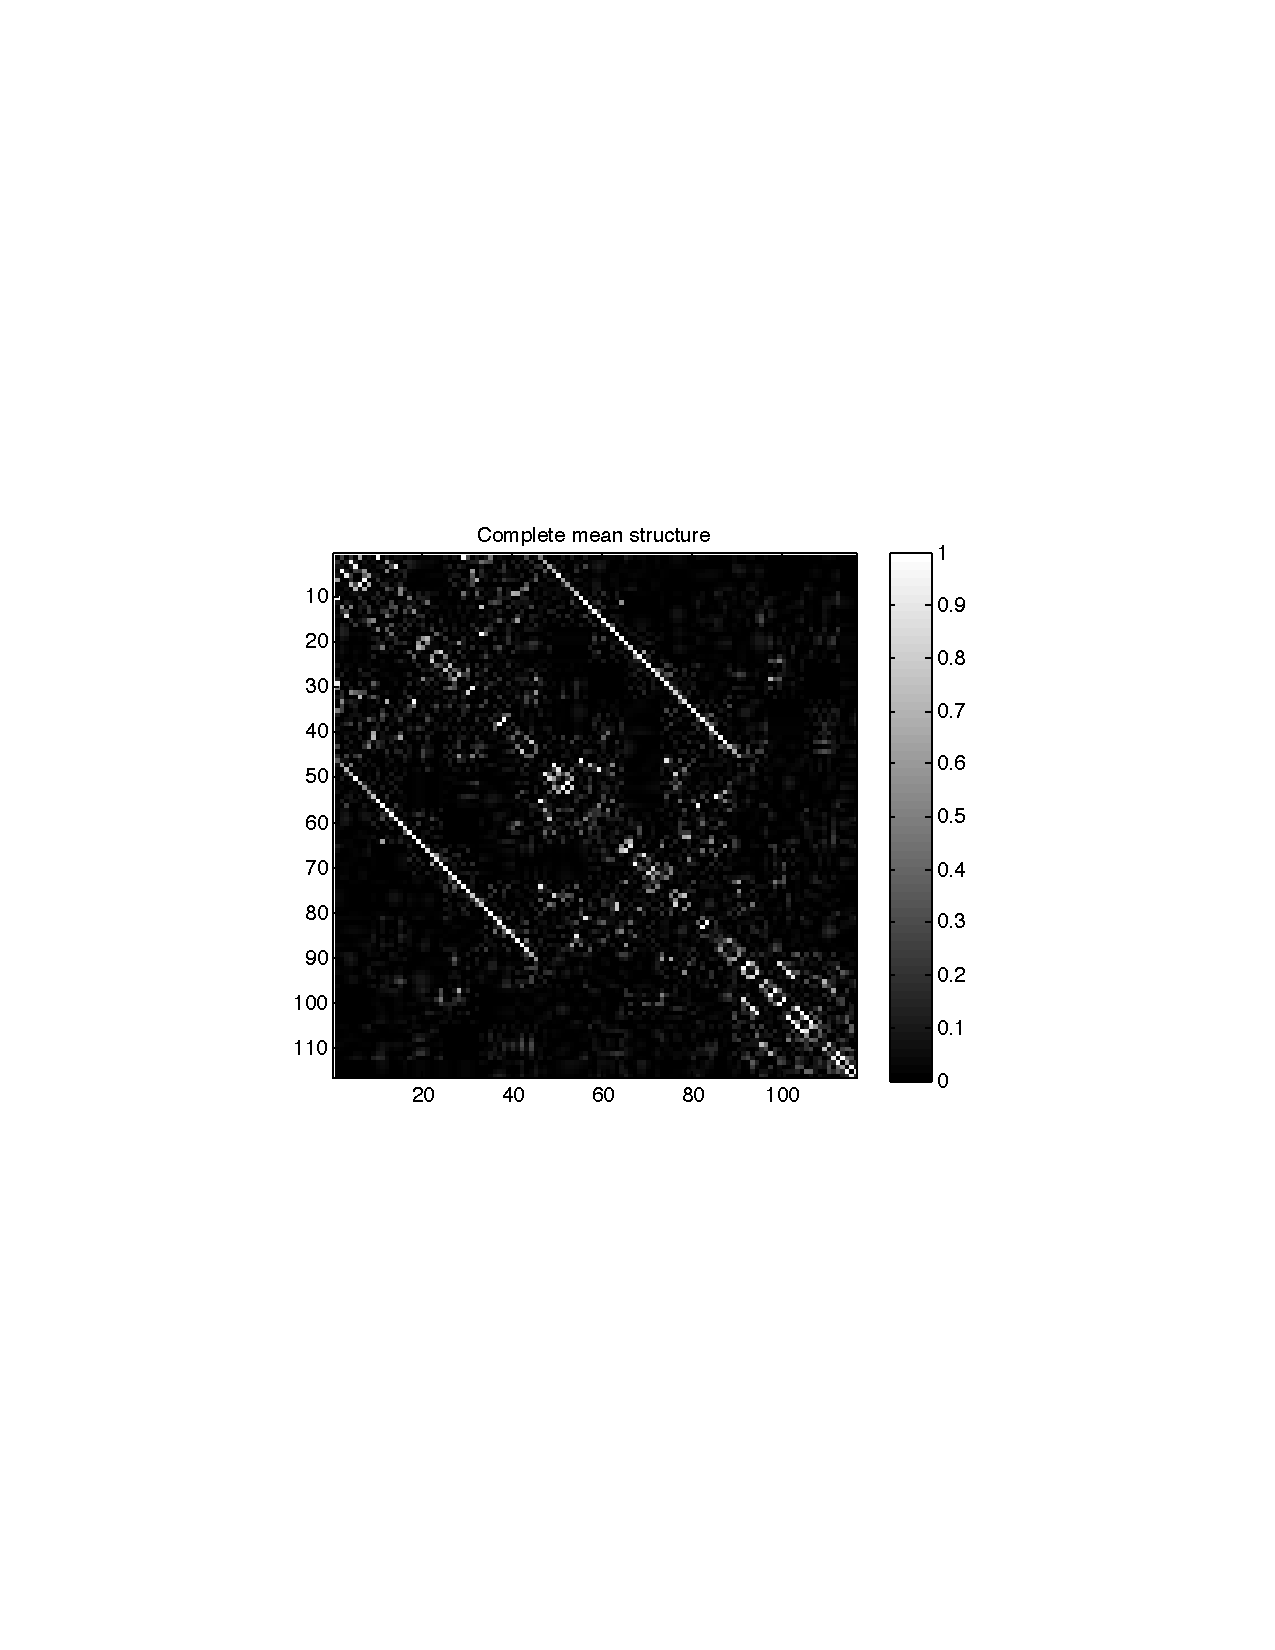
\includegraphics{images/struct_full_mean_gray}
  \caption{The avarage structure of all subjects, found with the PC-algorithm}
  \label{fig:struct_avg}
\end{figure}
In this matrix, higher values represent strong certainties of the presence of a connection.

\begin{figure}[h!]
  \centering
  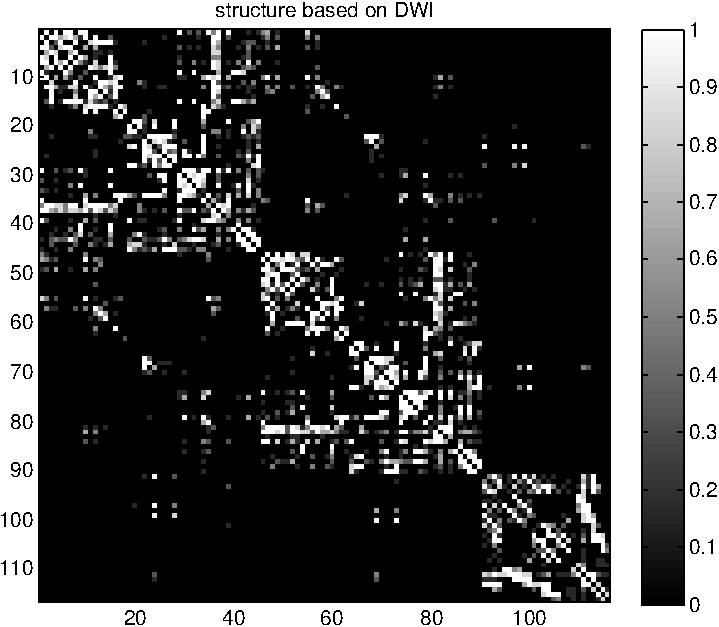
\includegraphics{images/structure_max}
  \caption{The avarage structure of all subjects, according to the DWI-measurements of Hinne et al.}
  \label{fig:struct_max}
\end{figure}


One notable difference between the results found in Hinne et al. is the strong connections between homological areas, visible as two diagonal lines.
This is a known shortcoming of diffusion weighted imaging, as these connections are typically too long to measure correctly.
These connections most likely correspond to the corpus callosum, as each region is connected with its counterpart in the other hemisphere..
Connections within the hemispheres are less clearly visible, as well as connections within the cerebellum.

The second step of the PC-algorithm finds directions based on this structure.
In Figures ~\ref{fig:pdag_avg_mod} and ~\ref{fig:pdag_avg_ems}, the results for both modified PC and EMS-PC are presented.
The figures look very similar to Figure ~\ref{fig:struct_avg}, and look strongly symmetric.
In terms of causality, this means that many latent sources are still present and causal relations between the measured brain regions themselves are not clearly visible.

\begin{figure}[h!]
  \centering
  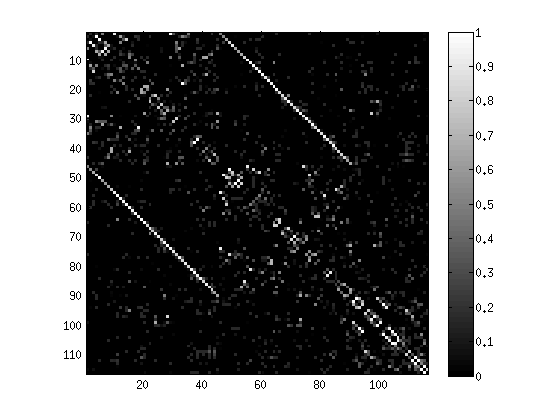
\includegraphics{images/PDAG_avg_mod}
  \caption{The PDAG found with modified PC, in which a high value denotes a high certainty of an arrow. The avarage of all six subjects is taken.}
  \label{fig:pdag_avg_mod}
\end{figure}

\begin{figure}[h!]
  \centering
  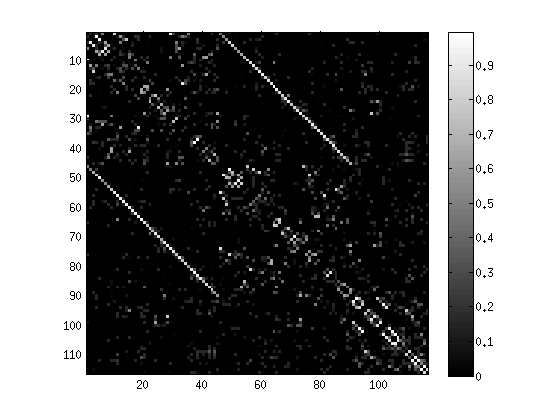
\includegraphics{images/PDAG_avg_expl}
  \caption{The PDAG found with EMS-PC, in which a high value denotes a high certainty of an arrow. The avarage of all six subjects is taken.}
  \label{fig:pdag_avg_ems}
\end{figure}

Another representation of this data has been used to emphasize the assymetric parts of Figures ~\ref{fig:pdag_avg_mod} and ~\ref{fig:pdag_avg_ems}.
To achieve this, the absolute difference between these matrices and their transpose has been calculated, lifting out those points for which there is an arrow in one direction, but not in the opposite direction.
These results are presented in Figures ~\ref{fig:pdag_avg_antisymmetric_mod} and ~\ref{fig:pdag_avg_antisymmetric_ems}.

\begin{figure}[h!]
  \centering
  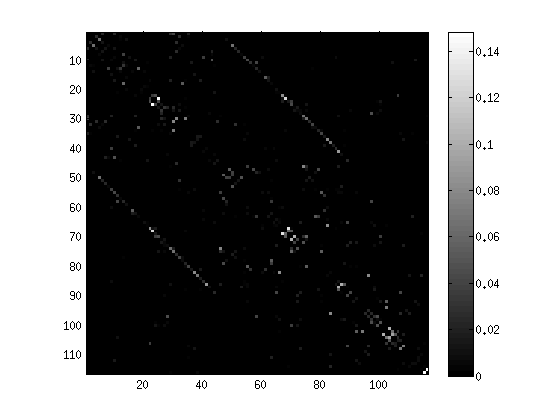
\includegraphics{images/PDAG_avg_antisymmetric_mod}
  \caption{The assymetric parts of the PDAG found with modified PC, in which a high value denotes a high certainty of an one-directional arrow. The avarage of all six subjects is taken.}
  \label{fig:pdag_avg_antisymmetric_mod}
\end{figure}

\begin{figure}[h!]
  \centering
  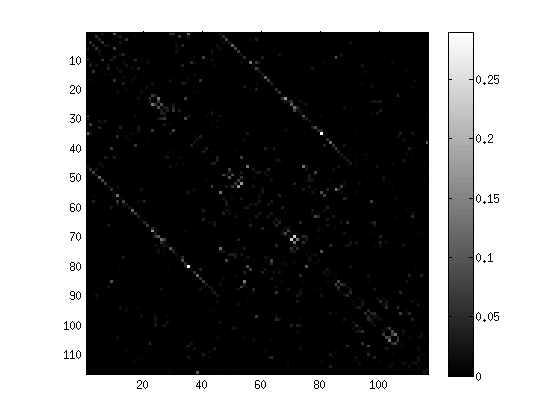
\includegraphics{images/PDAG_avg_antisymmetric_expl}
  \caption{The assymetric parts of the PDAG found with EMS-PC, in which a high value denotes a high certainty of an one-directional arrow. The avarage of all six subjects is taken.}
  \label{fig:pdag_avg_antisymmetric_ems}
\end{figure}

% iets over:
% hoogte van avg_antisymmetric, hoger bij EMS dus meer richting, maar bij beiden niet zo consistent over proefpersonen
% verschillen tussen beide hemispheres: niet zo logisch lijkt me, hemisphers zouden intern ongeveer hetzelfde moeten functioneren
% veel hoge waarden in 'blokjes' rond diagonaal, interessante dingen in de hemispheres?
% per proefpersoon maxima van ~0.5, maar een veel lager avarage over proefpersonen dus weinig consistentie

\section{Discussion}
% Further research
A Bayesian network cannot contain cycles, as that would imply that a variable is it's own ancestor and thus it's own cause.
The theory used here does not incorporate a temporal component and 
Ideally, a causal discovery methods finds only directed edges, resulting in a directed acyclic graph (DAG).
%In practice, however, often not all causal relations can be inferred and undirected edges are also used in a graph.
%As such, the result of a causal discovery method is a partially directed acyclic graph (PDAG).
As contemporary measuring techniques are too coarse and slow to model a brain at one point in time, correctly modelling variables over multiple points in time - opposing the acyclic assumption - would provide an interesting direction of further research.

% TODO: Suggereren task based analysis ipv resting state voor beter causaal beeld. 

\section{Conclusion}

\section{Acknowledgements}
We would like to thank Max Hinne and Tom Claassen, for without them this research would not have been viable.
They have provided us with ideas, valuable discussion and the data to perform actual research.

\bibliography{references}{}
\addcontentsline{toc}{section}{References}
\bibliographystyle{plain}

\end{document}